\documentclass[12pt]{ctexart}
\usepackage{amsfonts,amssymb}
\usepackage{float}
\usepackage{graphicx}
\usepackage{amsmath}
\usepackage{listings}
\usepackage{geometry}
\usepackage[usenames,dvipsnames]{xcolor}
\usepackage{setspace}
\geometry{a4paper}
\geometry{top=2cm} 
\geometry{bottom=2cm}
\geometry{left=0.5cm}
\geometry{right=1cm}

\title{微分方程数值解~项目作业 3}
\author{凌子恒 \\ 信息与计算科学 3200102551}

\begin{document}

\maketitle

\subsection*{实现细节及解释}

传参使用 \texttt{valarray} 以简化向量运算。

定义 \texttt{solution} 类存放结果,使用 \texttt{operator()} 访问某点处的函数值。

对于所有的隐式方法,采用迭代法。迭代终止条件为单次变化不超过 $10^{-14}$ 或者迭代次数超过 $1000$。 

所有的求解方法均为 \texttt{IVP} 类的间接派生类。继承关系如图:

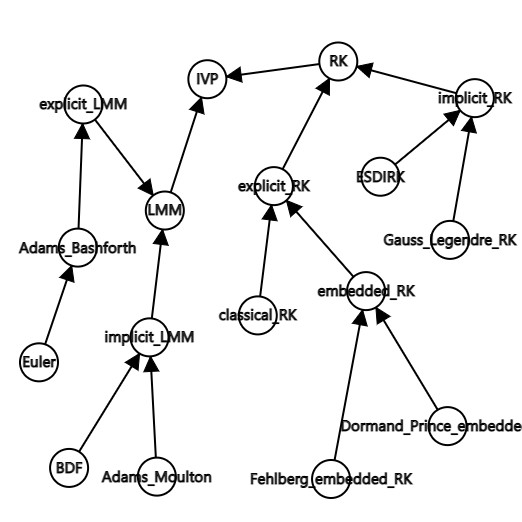
\includegraphics[scale=0.8]{1.jpg}

\texttt{factory.h} 提供了一个对象工厂类,通过输入的字符串返回类型为 \texttt{shared\_ptr<T>} 的基类指针。可以使用 \texttt{insert} 加入新派生类,使用 \texttt{erase} 删除派生类,使用 \texttt{operator[]} 查询某个字符串对应的派生类。若不存在,会抛出 \texttt{invalid\_argument}。(注:为编码方便,未使用要求中的名称,但原理效果是相同的)

注意代码运行总时间可能较长(可能达到数十分钟),不建议同时测试多个函数。

\subsection*{误差分析(11.199)}

代码见 \texttt{error1} 函数,从 \texttt{error1.in} 读入输出到 \texttt{error1.out}。\texttt{error1.in} 由 \texttt{data\_gen.py} 生成。

主要数据表格如下:

\begin{tabular}{c|c|c|c|c|c|c}
名字&$N$&误差 $1$&用时 $1$&误差 $2$&用时 $2$&收敛阶\\
\texttt{Adams-Bashforth(1)}&$500000$&$1.73e+00$&$0.191$&$1.64e+00$&$0.337$&$0.078$\\
\texttt{Adams-Bashforth(2)}&$500000$&$8.29e-01$&$0.656$&$1.97e-01$&$1.354$&$2.073$\\
\texttt{Adams-Bashforth(3)}&$500000$&$3.82e-03$&$0.861$&$4.96e-04$&$2.058$&$2.946$\\
\texttt{Adams-Bashforth(4)}&$500000$&$4.40e-04$&$1.103$&$2.80e-05$&$2.401$&$3.973$\\
\texttt{Adams-Moulton(2)}&$500000$&$1.38e-01$&$0.161$&$3.63e-02$&$0.301$&$1.924$\\
\texttt{Adams-Moulton(3)}&$500000$&$4.34e-04$&$0.678$&$5.60e-05$&$1.347$&$2.954$\\
\texttt{Adams-Moulton(4)}&$500000$&$3.35e-05$&$0.944$&$2.05e-06$&$1.941$&$4.033$\\
\texttt{Adams-Moulton(5)}&$100000$&$7.41e-04$&$0.317$&$1.18e-05$&$0.639$&$5.968$\\
\texttt{BDF(1)}&$500000$&$2.03e+00$&$0.229$&$2.01e+00$&$0.325$&$0.017$\\
\texttt{BDF(2)}&$500000$&$4.30e-01$&$0.689$&$1.37e-01$&$1.303$&$1.648$\\
\texttt{BDF(3)}&$500000$&$2.44e-03$&$0.952$&$3.23e-04$&$2.051$&$2.917$\\
\texttt{BDF(4)}&$500000$&$2.46e-04$&$1.238$&$4.95e-06$&$2.728$&$5.633$\\
\texttt{classical RK}&$500000$&$8.12e-07$&$0.150$&$5.20e-08$&$0.297$&$3.963$\\
\texttt{ESDIRK}&$500000$&$3.11e-07$&$0.932$&$1.99e-08$&$1.573$&$3.968$\\
\texttt{Gauss-Legendre RK(1)}&$500000$&$1.66e-01$&$0.140$&$3.96e-02$&$0.285$&$2.068$\\
\texttt{Gauss-Legendre RK(2)}&$500000$&$2.04e-07$&$0.252$&$1.32e-08$&$0.487$&$3.955$\\
\texttt{Gauss-Legendre RK(3)}&$20000$&$4.00e-04$&$0.021$&$6.18e-06$&$0.035$&$6.014$\\
\texttt{Fehlberg embedded RK}&$200000$&$3.72e-06$&$0.086$&$2.21e-07$&$0.166$&$4.069$\\
\texttt{Dormand-Prince embedded RK}&$20000$&$9.91e-04$&$0.009$&$3.60e-05$&$0.018$&$4.782$\\
\end{tabular}

其中,$1$ 为 $step=N$,$2$ 为 $step=2N$。这里为一些算法设置了特殊的 $N$ 以提高效率及降低机器精度带来的影响。

\subsection*{误差分析(11.200)}

代码见 \texttt{error2} 函数,从 \texttt{error2.in} 读入输出到 \texttt{error2.out}。\texttt{error2.in} 由 \texttt{data\_gen.py} 生成。

主要数据表格如下:

\begin{tabular}{c|c|c|c|c|c|c}
名字&$N$&误差 $1$&用时 $1$&误差 $2$&用时 $2$&收敛阶\\
\texttt{Adams-Bashforth(1)}&$50000$&$5.33e-01$&$0.018$&$2.20e-01$&$0.029$&$1.278$\\
\texttt{Adams-Bashforth(2)}&$50000$&$2.61e-04$&$0.058$&$6.80e-05$&$0.134$&$1.940$\\
\texttt{Adams-Bashforth(3)}&$50000$&$3.33e-05$&$0.085$&$4.16e-06$&$0.204$&$2.999$\\
\texttt{Adams-Bashforth(4)}&$50000$&$3.79e-09$&$0.105$&$1.98e-10$&$0.242$&$4.261$\\
\texttt{Adams-Moulton(2)}&$50000$&$5.66e-05$&$0.019$&$1.42e-05$&$0.044$&$2.000$\\
\texttt{Adams-Moulton(3)}&$50000$&$3.70e-06$&$0.071$&$4.62e-07$&$0.179$&$3.000$\\
\texttt{Adams-Moulton(4)}&$5000$&$1.87e-06$&$0.018$&$6.97e-08$&$0.031$&$4.742$\\
\texttt{Adams-Moulton(5)}&$1000$&$1.42e-02$&$0.004$&$5.07e-04$&$0.007$&$4.805$\\
\texttt{BDF(1)}&$50000$&$8.42e-01$&$0.028$&$3.90e-01$&$0.050$&$1.110$\\
\texttt{BDF(2)}&$50000$&$2.04e-04$&$0.089$&$5.38e-05$&$0.155$&$1.924$\\
\texttt{BDF(3)}&$5000$&$2.34e-02$&$0.015$&$2.79e-03$&$0.028$&$3.067$\\
\texttt{BDF(4)}&$5000$&$6.41e-05$&$0.016$&$1.04e-06$&$0.034$&$5.949$\\
\texttt{classical RK}&$5000$&$2.22e-07$&$0.001$&$5.21e-09$&$0.003$&$5.412$\\
\texttt{ESDIRK}&$5000$&$7.62e-08$&$0.015$&$3.45e-09$&$0.026$&$4.467$\\
\texttt{Gauss-Legendre RK(1)}&$5000$&$5.38e-03$&$0.002$&$1.34e-03$&$0.004$&$2.004$\\
\texttt{Gauss-Legendre RK(2)}&$5000$&$2.04e-07$&$0.004$&$1.27e-08$&$0.007$&$4.008$\\
\texttt{Gauss-Legendre RK(3)}&$2000$&$1.74e-09$&$0.003$&$4.67e-11$&$0.006$&$5.221$\\
\texttt{Fehlberg embedded RK}&$2000$&$2.05e-05$&$0.001$&$5.90e-07$&$0.002$&$5.121$\\
\texttt{Dormand-Prince embedded RK}&$2000$&$1.34e-06$&$0.001$&$4.71e-08$&$0.002$&$4.829$\\
\end{tabular}

其中,$1$ 为 $step=N$,$2$ 为 $step=2N$。这里为一些算法设置了特殊的 $N$ 以提高效率及降低机器精度带来的影响。

\subsection*{作图}

计算坐标见 plot 函数,从 plot.in 读入输出到 Euler.in 等文件。plot.py 实现了画图,结果如下:

Euler:

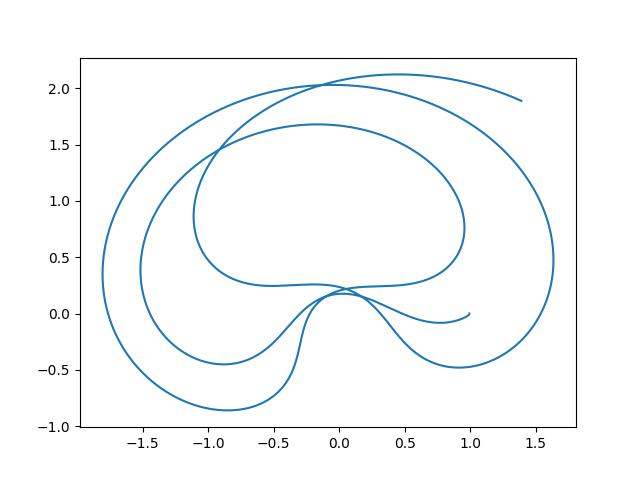
\includegraphics[scale=0.8]{Euler.jpg}

classical RK:

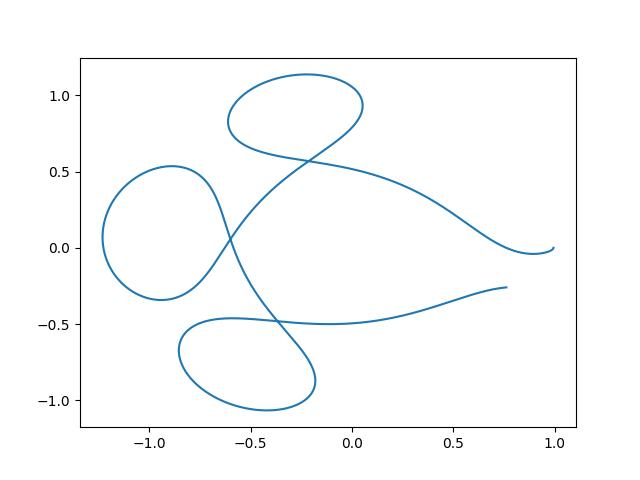
\includegraphics[scale=0.8]{classical RK.jpg}

Dormand-Prince embedded RK:

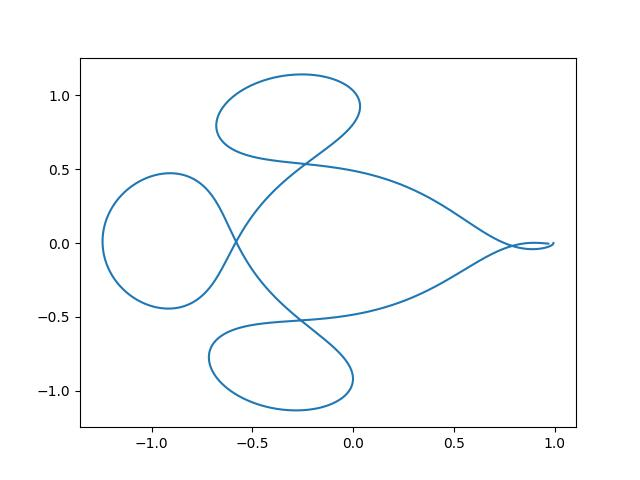
\includegraphics[scale=0.8]{Dormand-Prince embedded RK.jpg}

\subsection*{(c)}

由于图像接近较为主观,这里手动测试,认为分 $N$ 段时,图像较为接近。

\begin{tabular}{c|c|c}
	名称&$N$ (11.119) &$N$ (11.120) \\
	Adams-Bashforth(1)&$3\times 10^6$&$7\times 10^6$\\
	Adams-Bashforth(2)&$2\times 10^5$&$4\times 10^3$\\
	Adams-Bashforth(3)&$3\times 10^4$&$8\times 10^3$\\
	Adams-Bashforth(4)&$5\times 10^4$&$2\times 10^3$\\
	Adams-Moulton(2)&$2\times 10^5$&$3\times 10^3$\\
	Adams-Moulton(3)&$2\times 10^4$&$4\times 10^3$\\
	Adams-Moulton(4)&$3\times 10^4$&$9\times 10^2$\\
	Adams-Moulton(5)&$1\times 10^4$&$1\times 10^3$\\
	BDF(1)&$5\times 10^6$&$5\times 10^6$\\
	BDF(2)&$3\times 10^5$&$4\times 10^3$\\
	BDF(3)&$4\times 10^4$&$6\times 10^3$\\
	BDF(4)&$4\times 10^4$&$2\times 10^3$\\
	classical RK&$2\times 10^4$&$8\times 10^2$\\
	ESDIRK&$9\times 10^3$&$9\times 10^3$\\
	Gauss-Legendre RK(1)&$9\times 10^4$&$3\times 10^3$\\
	Gauss-Legendre RK(2)&$7\times 10^3$&$3\times 10^2$\\
	Gauss-Legendre RK(3)&$4\times 10^3$&$2\times 10^2$\\
	Fehlberg embedded RK&$7\times 10^3$&$5\times 10^2$\\
	Dormand-Prince embedded RK&$7\times 10^3$&$4\times 10^2$\\
\end{tabular}

\subsection*{$10^{-3}$ 下速度比较}

首先,去除难以到 $10^{-3}$ 精度的五种低阶方法。

由 \texttt{data\_gen.py} 生成输入文件 \texttt{bsearch.in},由 \texttt{bsearch} 函数从 \texttt{bsearch.in} 读入输出到 \texttt{bsearch.out}。

函数原理是先倍增到可以满足精度要求,再二分最小的 step。由于运行较慢,考虑做一个粗略的二分,并计算两端点用时确定运行时间区间。 

观察输出结果,可以发现 (11.119) 中 Dormand-Prince embedded RK 优于其余所有,而 (11.120) 中 Dormand-Prince embedded RK 和 Fehlberg embedded RK 时间区间有交,无法判断。

进一步只测试这两个方法(见 \texttt{bsearch2} 相关文件),Dormand-Prince embedded RK 仍然用时更少。

故在两例中 Dormand-Prince embedded RK 均更优秀。

\end{document}
